\chapter{\textsc{Project Design}}
\label{chapter:project_design}

As a result of the project design phase, the problem statement and objectives were established, while the motivation behind the project was defined. A high-level sense of the methodology employed is also presented, together with a flow-chart created during the project planning phase.

\section{Problem statement}

The problem addressed in this project is concerned with the rational clustering of networks constructed using real data. This project focuses on identifying a solution to a real-world problem faced by EPSRC involving the definition of topic classifications. EPSRC is in possession of substantial grant data which can be used to formulate networks of \textit{topics} and \textit{researchers}. Ideally, the next step would involve the division of the networks created in order to obtain several groups of topics based on similarity or relatedness. The "best" group would represent the classification of its topics to a research area. This method would make the finer or coarser definition of topics significantly easier. However, as of yet, a way of achieving this has not been identified.

\section{Objectives and Motivation}

The overall aim of this project can be divided into three different objectives of diverse importance. Firstly, and most importantly, at the end of the project, a rational clustering of topics is expected to be produced using graph theory. Secondly, and equally as important, the project seeks to prove that a novel approach in graph theory can be employed to solve and provide a solution to the real-world problem addressed. Finally, this thesis project also aims to demonstrate that the novel approach can be applied to a different data set involved in the clustering of researchers.

Furthermore, the motivation behind this thesis project is primarily fuelled by the real-world aspect of the problem considered. Personally, I believe that contributing towards something that may be beneficial to other people adds enthusiasm which translates into a more efficient work rate and higher standard of quality.

Originally, the concept of the project came from Dr. Shi Zhou, the supervisor of this thesis project. Recently, he attended a talk where an EPSRC officer expressed concerns regarding the way research topics were defined. Therefore, the project was principally specific to one organisation and problem. However, with time, the data took on a new significance as the invaluable human judgement underlying it was discovered. This changed the aim of the project as it became a project concerned with a general real-world problem. In this new meaning, graph theory combined with the human judgement behind the links connecting the topics in a network is used to identify an optimal way of clustering topics meaningfully. 

\section{Methodology}

This project uses current and historical data publicly provided by EPSRC through the EPSRC Grants on the Web (GoW) service. Networks of \textit{Topics} and \textit{Researchers} are constructed using the data collected from EPSRC. Node and edge attributes are also formulated, and the attribute values normalised. This is followed by extensive comparison experiments on two different interpretations of the two types of networks considering three different edge weight interpretations and eight different community detection algorithms. The three edge weight interpretations are \textit{unweighted}, \textit{weighted by the normalised number of grants} and \textit{weighted by the normalised value of grants}, while community detection algorithms include \textit{Spinglass}, \textit{Louvain} and \textit{Fast Greedy}. Subsequently, the topic and researcher clusters are evaluated by calculating the average Dice and Jaccard similarity of node pairs between and within the clusters. The results of the experiments are expected to represent the identification of an optimal combination of edge weight and community detection algorithm which produces a coherent, balanced and well-defined clustering of topics and researchers.

\clearpage

\section{Project Plan}

Prior to development and analysis stages, a plan was produced in the form of a flow chart, presented in Fig. \ref{fig:flow_chart}, which details every major process that was completed in order to achieve the objectives set in the Project Design.

\begin{figure}[htpb]
    \centering
    \fbox{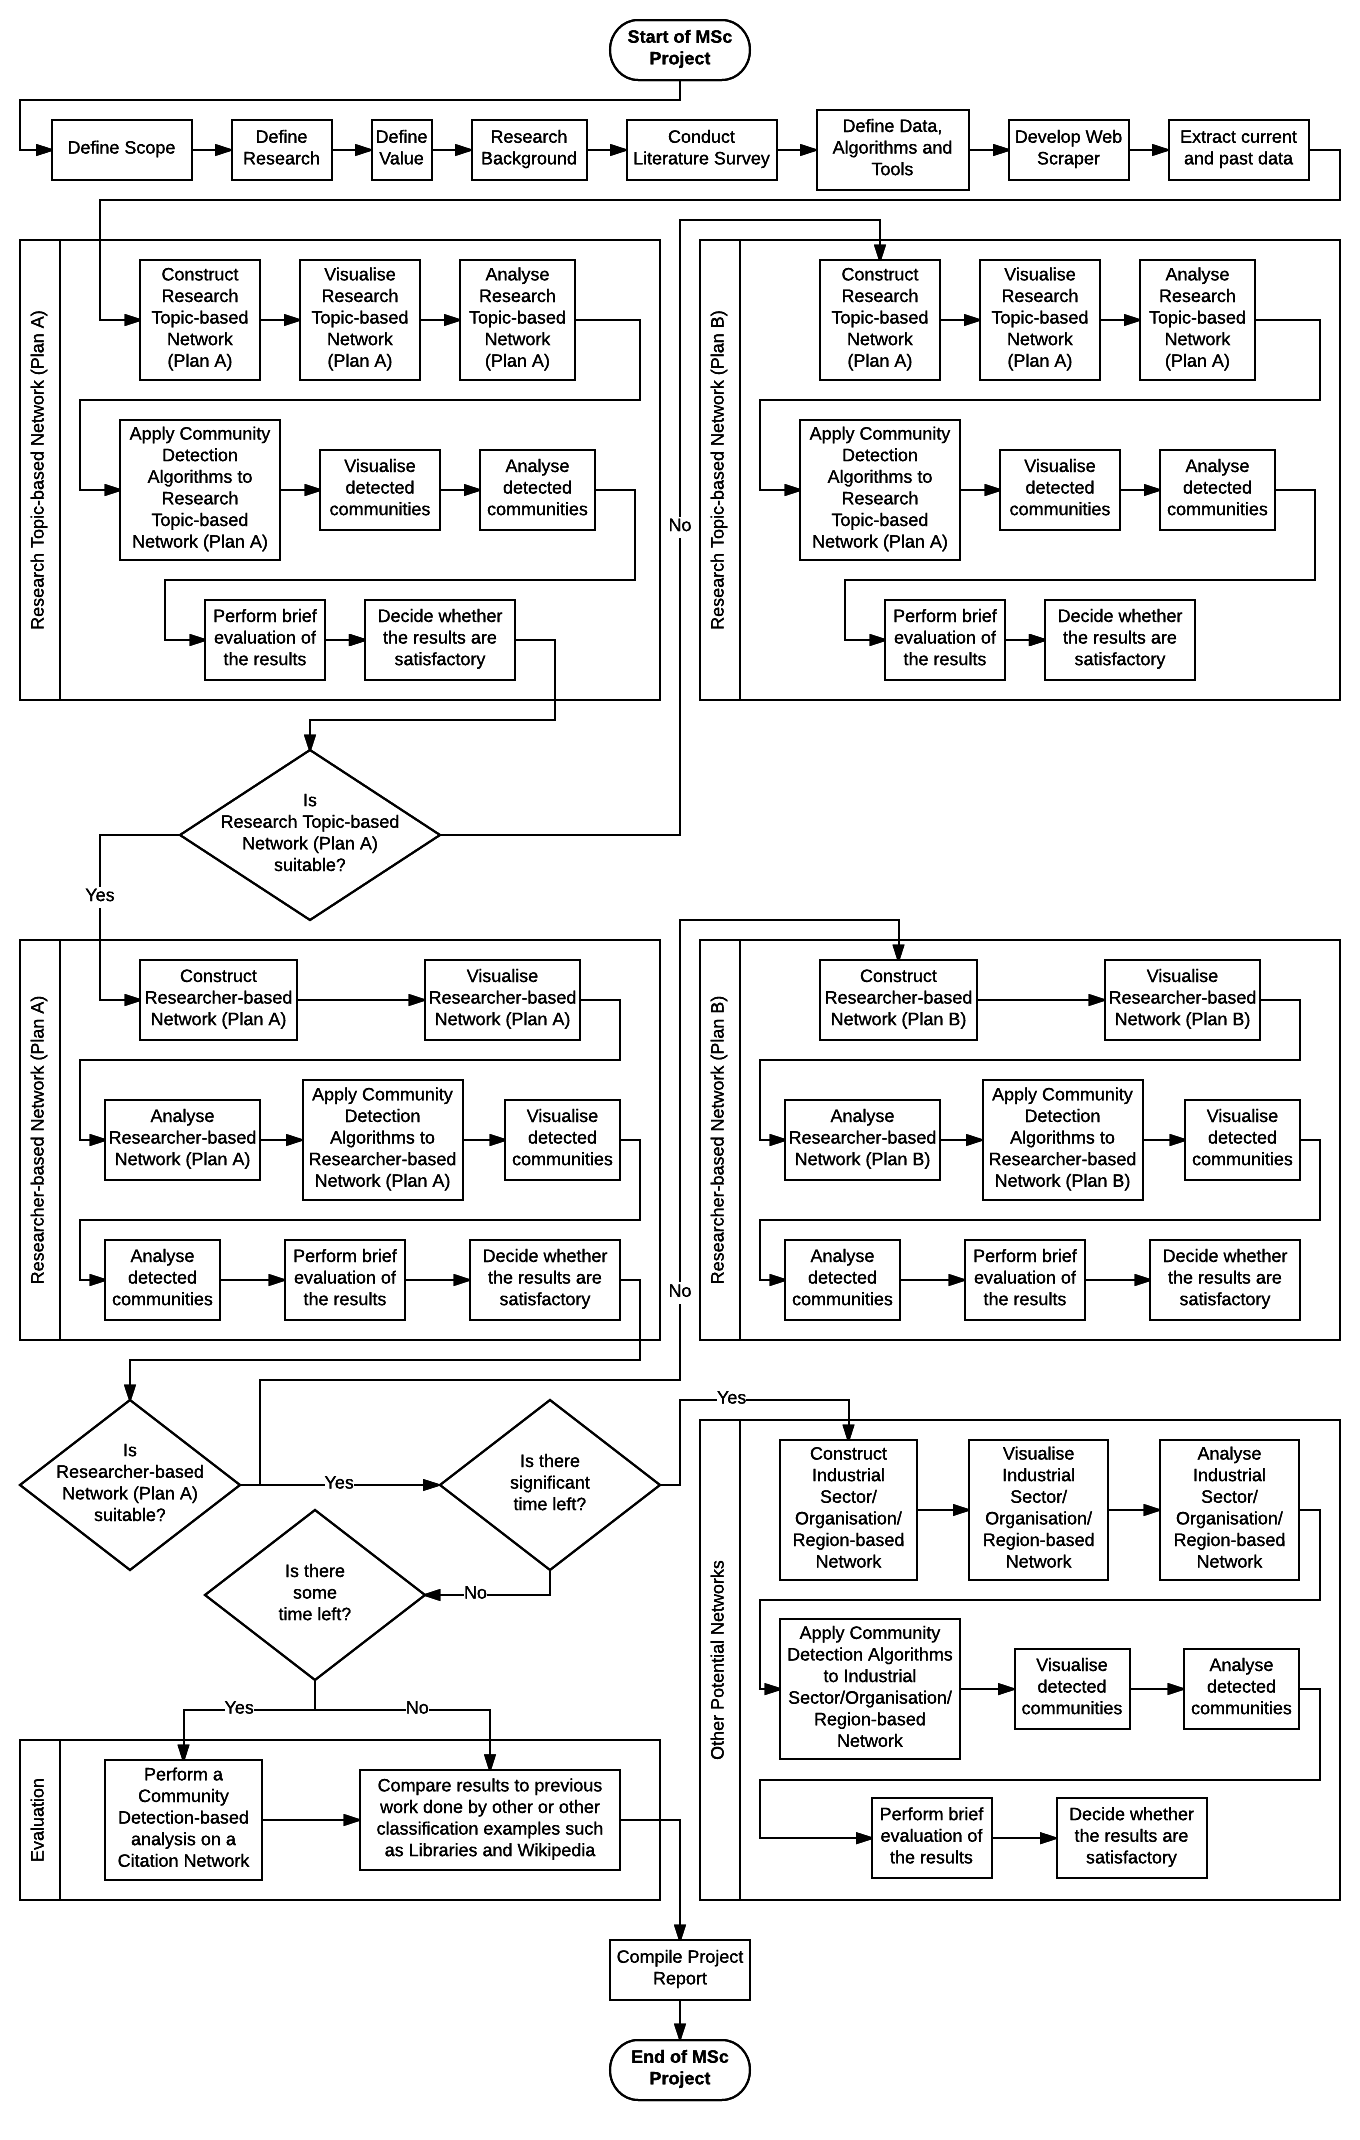
\includegraphics[width=11.5cm]{flow-charts/flow_chart}}
    \caption{Flow chart created as part of the Project Plan, showing the transition between the different stages of the project.}
    \label{fig:flow_chart}
\end{figure}

\clearpage